\documentclass[11pt,spanish]{article}

\input{preamble.tex}
\newcommand{\namestudent}{Americo Ignacio Acuña Rodriguez}
\newcommand{\rolusm}{202473037-7}
\newcommand{\campus}{Casa Central}
\newcommand{\authorcity}{Valparaíso}
\newcommand{\tnum}{1}
\newcommand{\sem}{2026-2}
\newcommand{\repourl}{https://github.com/Ameripro2006/INF221_T1_2026-2}

\headheight=14pt
\linespread{1.15}

\title{
  \huge
  \textbf{REPORTE TAREA \tnum~ \\ ALGORITMOS Y COMPLEJIDAD} \\[1ex]
  \emph{\textquote{Más allá de la notación asintótica: Análisis experimental de algoritmos de ordenamiento y multiplicación de matrices.}}
}

\author{\namestudent}


\begin{document}
\maketitle

\pagestyle{fancy}
\fancyhf{}
\chead{REPORTE TAREA \tnum~}
\rhead{\sem}
\lhead{INF-221}
\fancyfoot[L]{Campus \campus \\ \authorcity}
\fancyfoot[C]{\thepage}
\fancyfoot[R]{\namestudent \\ \rolusm}
\renewcommand{\headrulewidth}{0.4pt}
\renewcommand{\footrulewidth}{0.4pt}
\thispagestyle{fancy}

\vspace{-1.0\baselineskip}

\begin{abstract}
El presente reporte evalúa el comportamiento empírico de algoritmos fundamentales de ordenamiento (\texttt{MergeSort}, \texttt{QuickSort}, \texttt{PatienceSort} y \texttt{std::sort}) y multiplicación matricial (algoritmo clásico \textit{Naive} frente a \textit{Strassen}). Mediante experimentación sistemática sobre hardware AMD Ryzen y Linux, se contrasta la teoría de complejidad asintótica frente al rendimiento real influenciado por la jerarquía de memorias caché, asignación dinámica y optimizaciones del compilador.
\end{abstract}

\section{Introducción}
El análisis asintótico tradicional clasifica algoritmos según su crecimiento teórico, omitiendo restricciones de hardware como la jerarquía de memorias o las optimizaciones del compilador. Este estudio evalúa empíricamente dos problemas: el ordenamiento unidimensional (MergeSort, QuickSort, PatienceSort y \texttt{std::sort}) y la multiplicación de matrices cuadradas (Naive vs Strassen), contrastando la teoría formal frente al rendimiento práctico. El código fuente y los datos están disponibles en: \url{https://github.com/Ameripro2006/INF221_T1_2026-2}.

\section{Implementación y Repositorio}
Todo el código fuente desarrollado para las experiencias de ordenamiento y multiplicación matricial, junto con los generadores de casos de prueba y scripts de análisis estadístico en Python, se encuentra disponible de forma pública en el siguiente repositorio de GitHub:

\begin{center}
    \url{\repourl}
\end{center}

\section{Entorno experimental}
Los experimentos fueron ejecutados en una máquina bajo Linux (kernel 6.x) equipada con un procesador \textbf{AMD Ryzen 5 7600X} (6 núcleos, 12 hilos, 4.7~GHz base / 5.3~GHz boost), tarjeta gráfica \textbf{AMD Radeon RX 6900 XT} (16~GB VRAM) y \textbf{32~GB de memoria RAM DDR5} en dual-channel ($2 \times 16\,\text{GB}$). El código se desarrolló en C++17 y fue compilado mediante \texttt{g++} con optimización \texttt{-O2}. Los tiempos de ejecución se registraron con \texttt{std::chrono::high\_resolution\_clock}.

Para ordenamiento, se evaluaron arreglos con tamaños $N \in \{10^1, 10^3, 10^5, 10^7\}$ bajo cuatro escenarios: secuencias aleatorias, ordenadas ascendentemente, ordenadas descendentemente y arreglos con dominios restringidos de valores. Para la multiplicación matricial, se utilizaron matrices cuadradas con dimensiones $N \in \{16, 64, 256, 1024\}$, variando su estructura interna (dispersas, diagonales y densas) y dominio numérico ($D_0 \in \{0, 1\}$ y $D_{10} \in [0, 10]$), con tres réplicas independientes por configuración.

\section{Resultados y Análisis}
\subsection{Algoritmos de Ordenamiento}
El análisis experimental expone una fuerte sensibilidad a la distribución inicial de los datos.

\begin{figure}[H]
    \centering
    \begin{minipage}{0.48\textwidth}
        \centering
        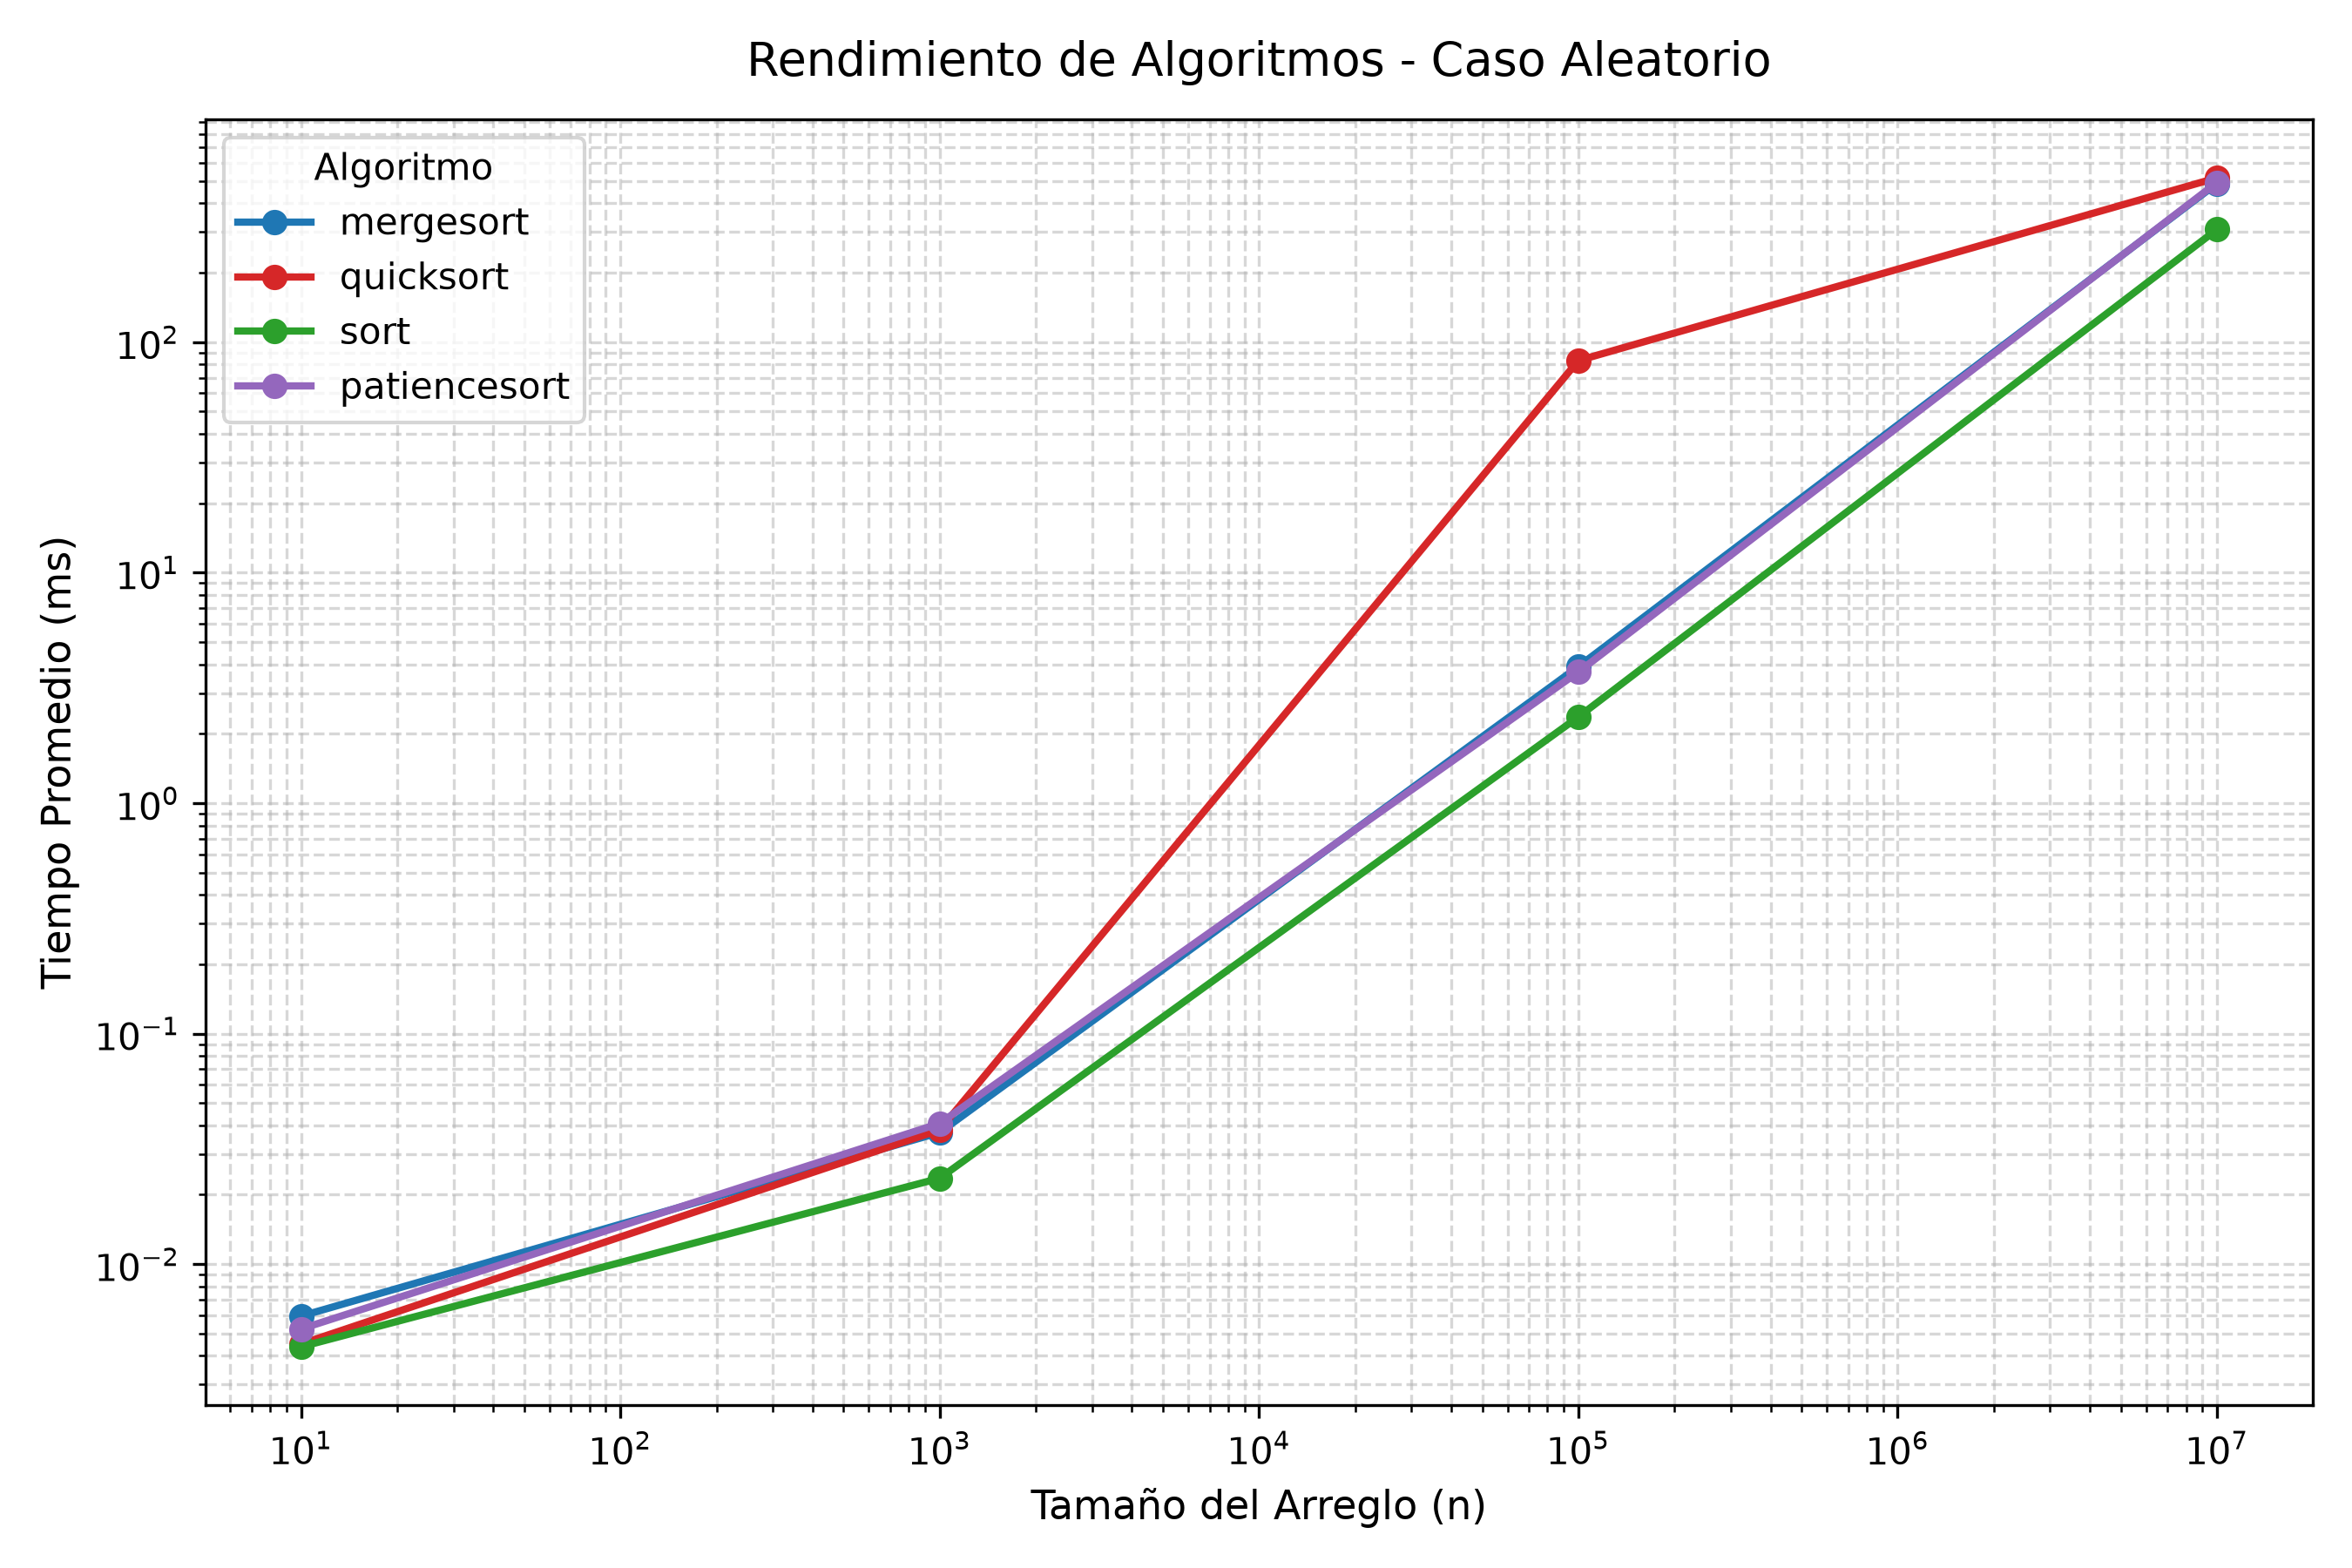
\includegraphics[width=\textwidth]{figures/comparativa_aleatorio.png}
        \caption{Tiempo: Caso aleatorio.}
        \label{fig:t_aleatorio}
    \end{minipage}\hfill
    \begin{minipage}{0.48\textwidth}
        \centering
        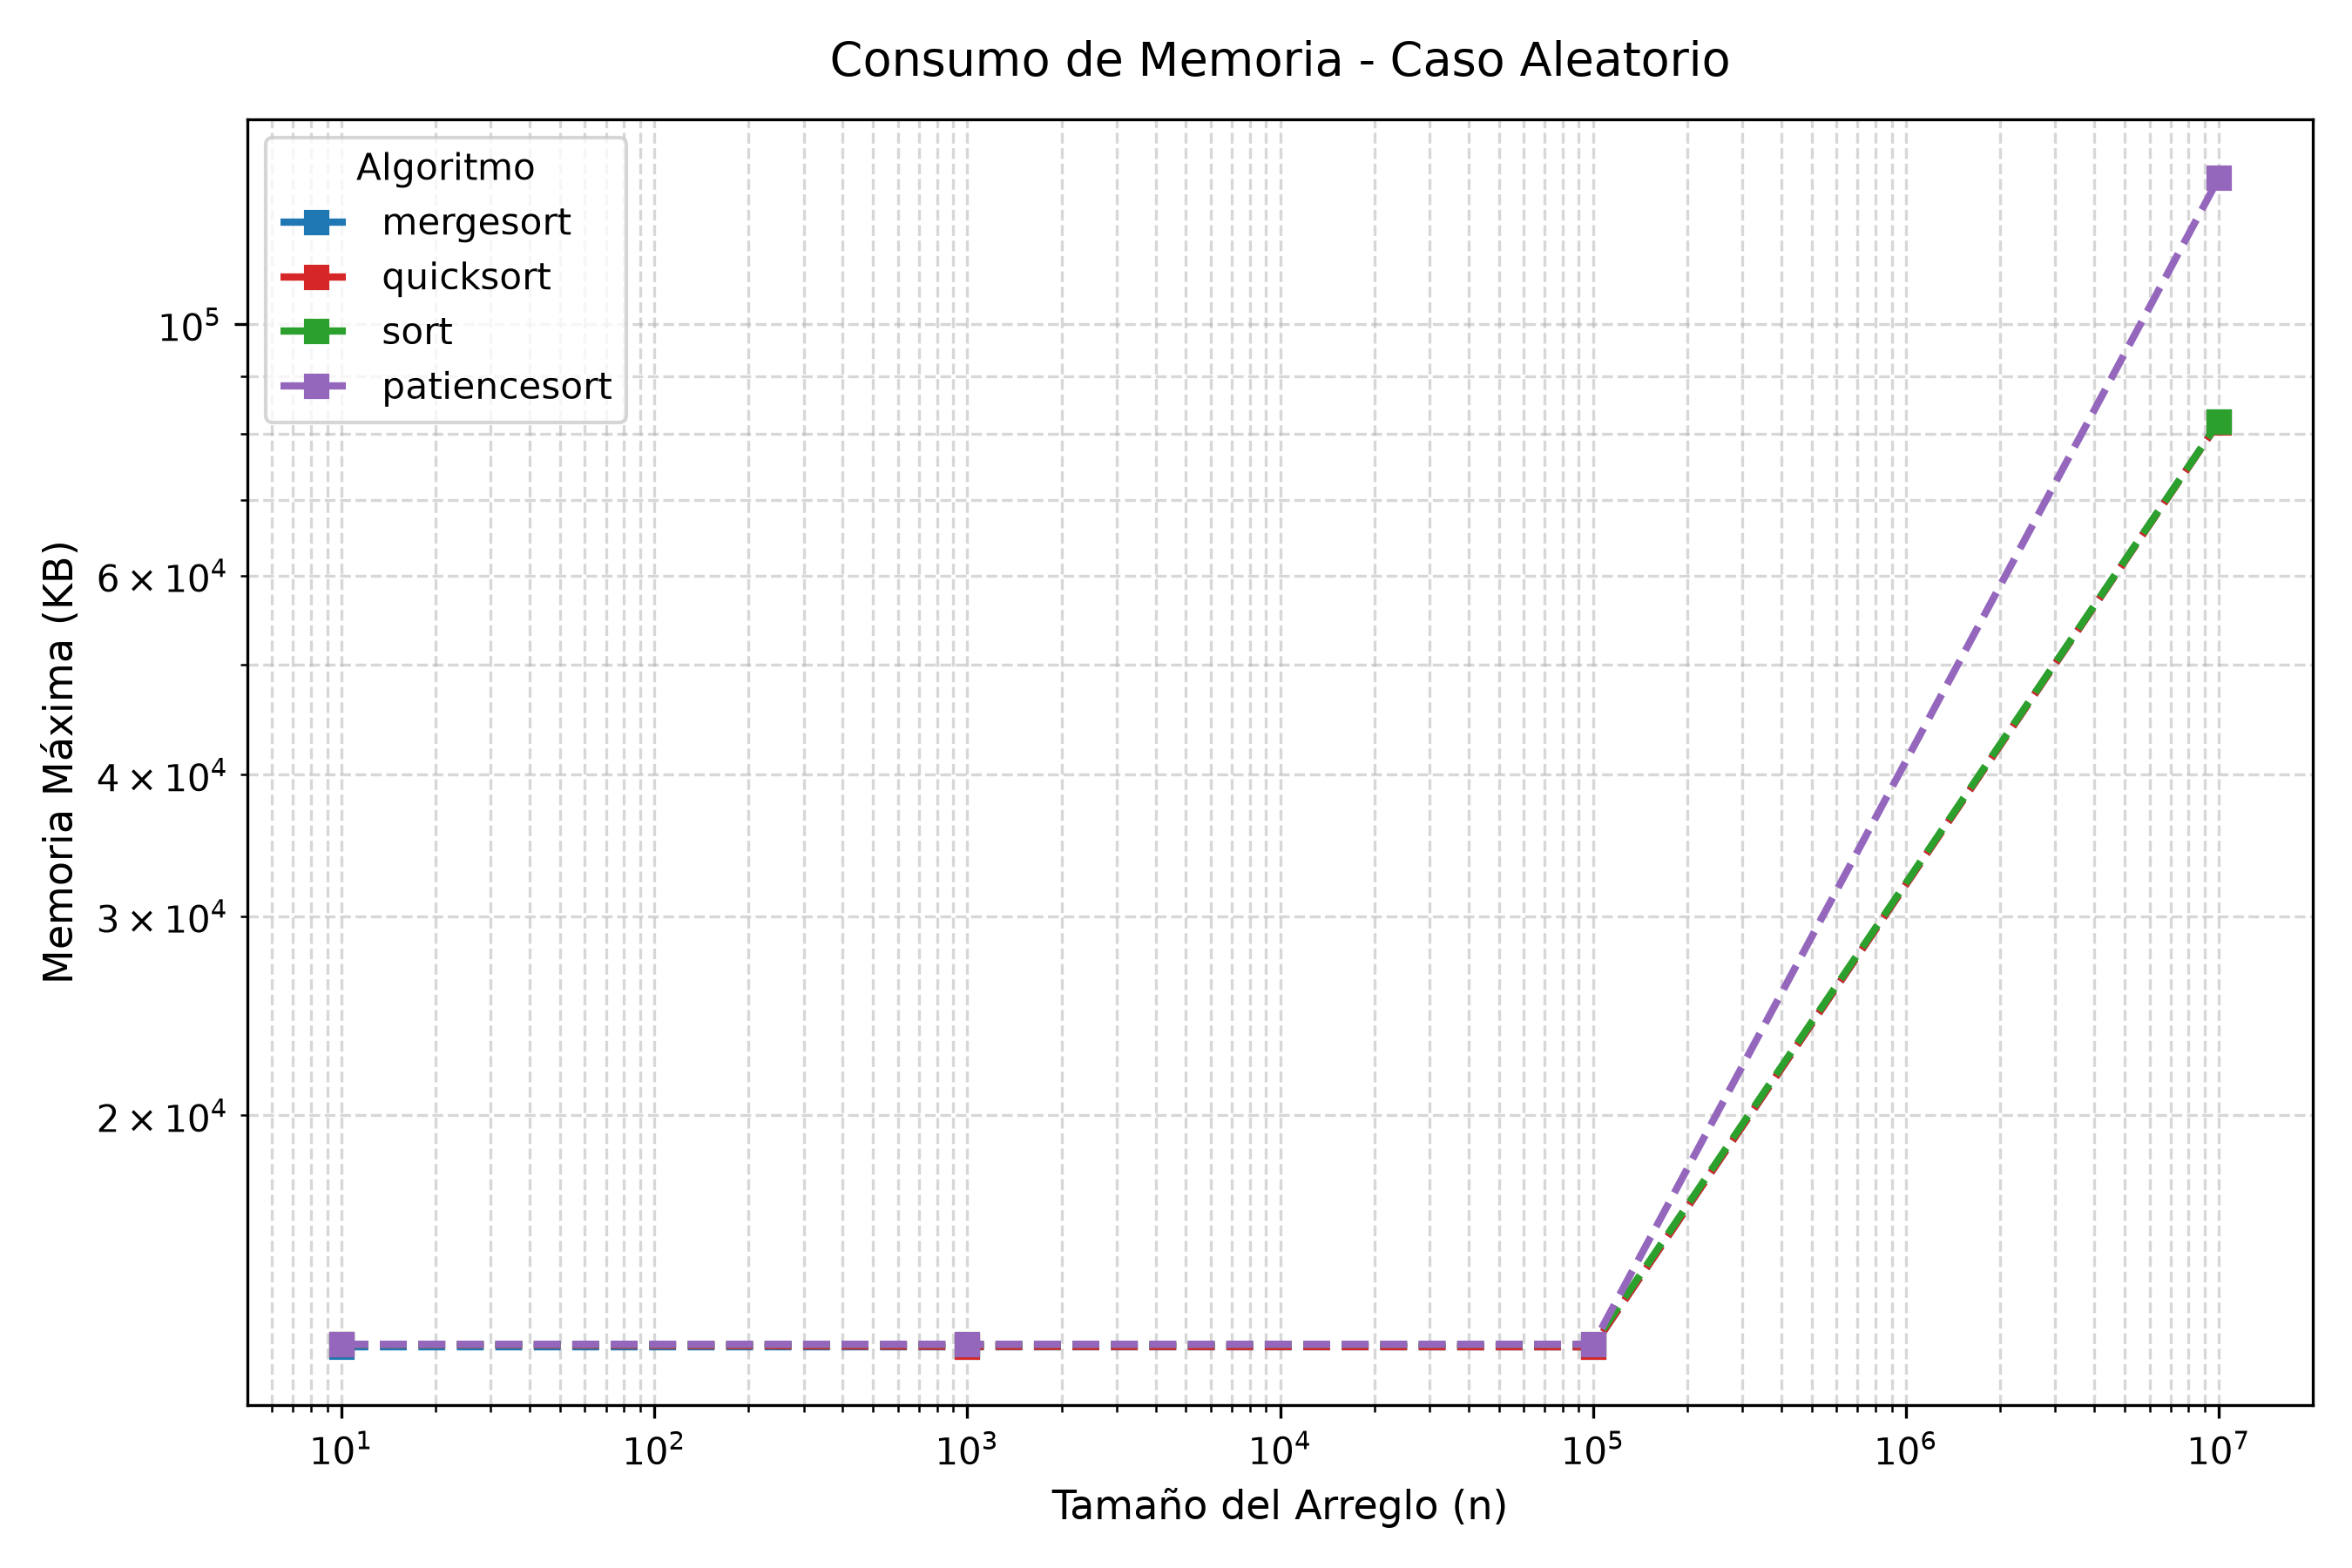
\includegraphics[width=\textwidth]{figures/memoria_aleatorio.png}
        \caption{Memoria: Caso aleatorio.}
        \label{fig:m_aleatorio}
    \end{minipage}
\end{figure}

En la Figura \ref{fig:t_aleatorio}, \texttt{std::sort} logra la menor latencia. QuickSort sufre una degradación catastrófica a $\mathcal{O}(N^2)$ con arreglos ordenados, consumiendo toda la pila (\textit{Stack Overflow}) o excediendo el límite de tiempo para $N \ge 10^6$. MergeSort conserva su tasa teórica $\mathcal{O}(N \log N)$, mientras que PatienceSort mantiene su cota pero con una alta constante multiplicativa. Respecto a la memoria (Figura \ref{fig:m_aleatorio}), \texttt{std::sort} domina operando \textit{in-place}, mientras MergeSort y PatienceSort exhiben un crecimiento $\mathcal{O}(N)$ por sus estructuras auxiliares.

\begin{figure}[H]
    \centering
    \begin{minipage}{0.32\textwidth}
        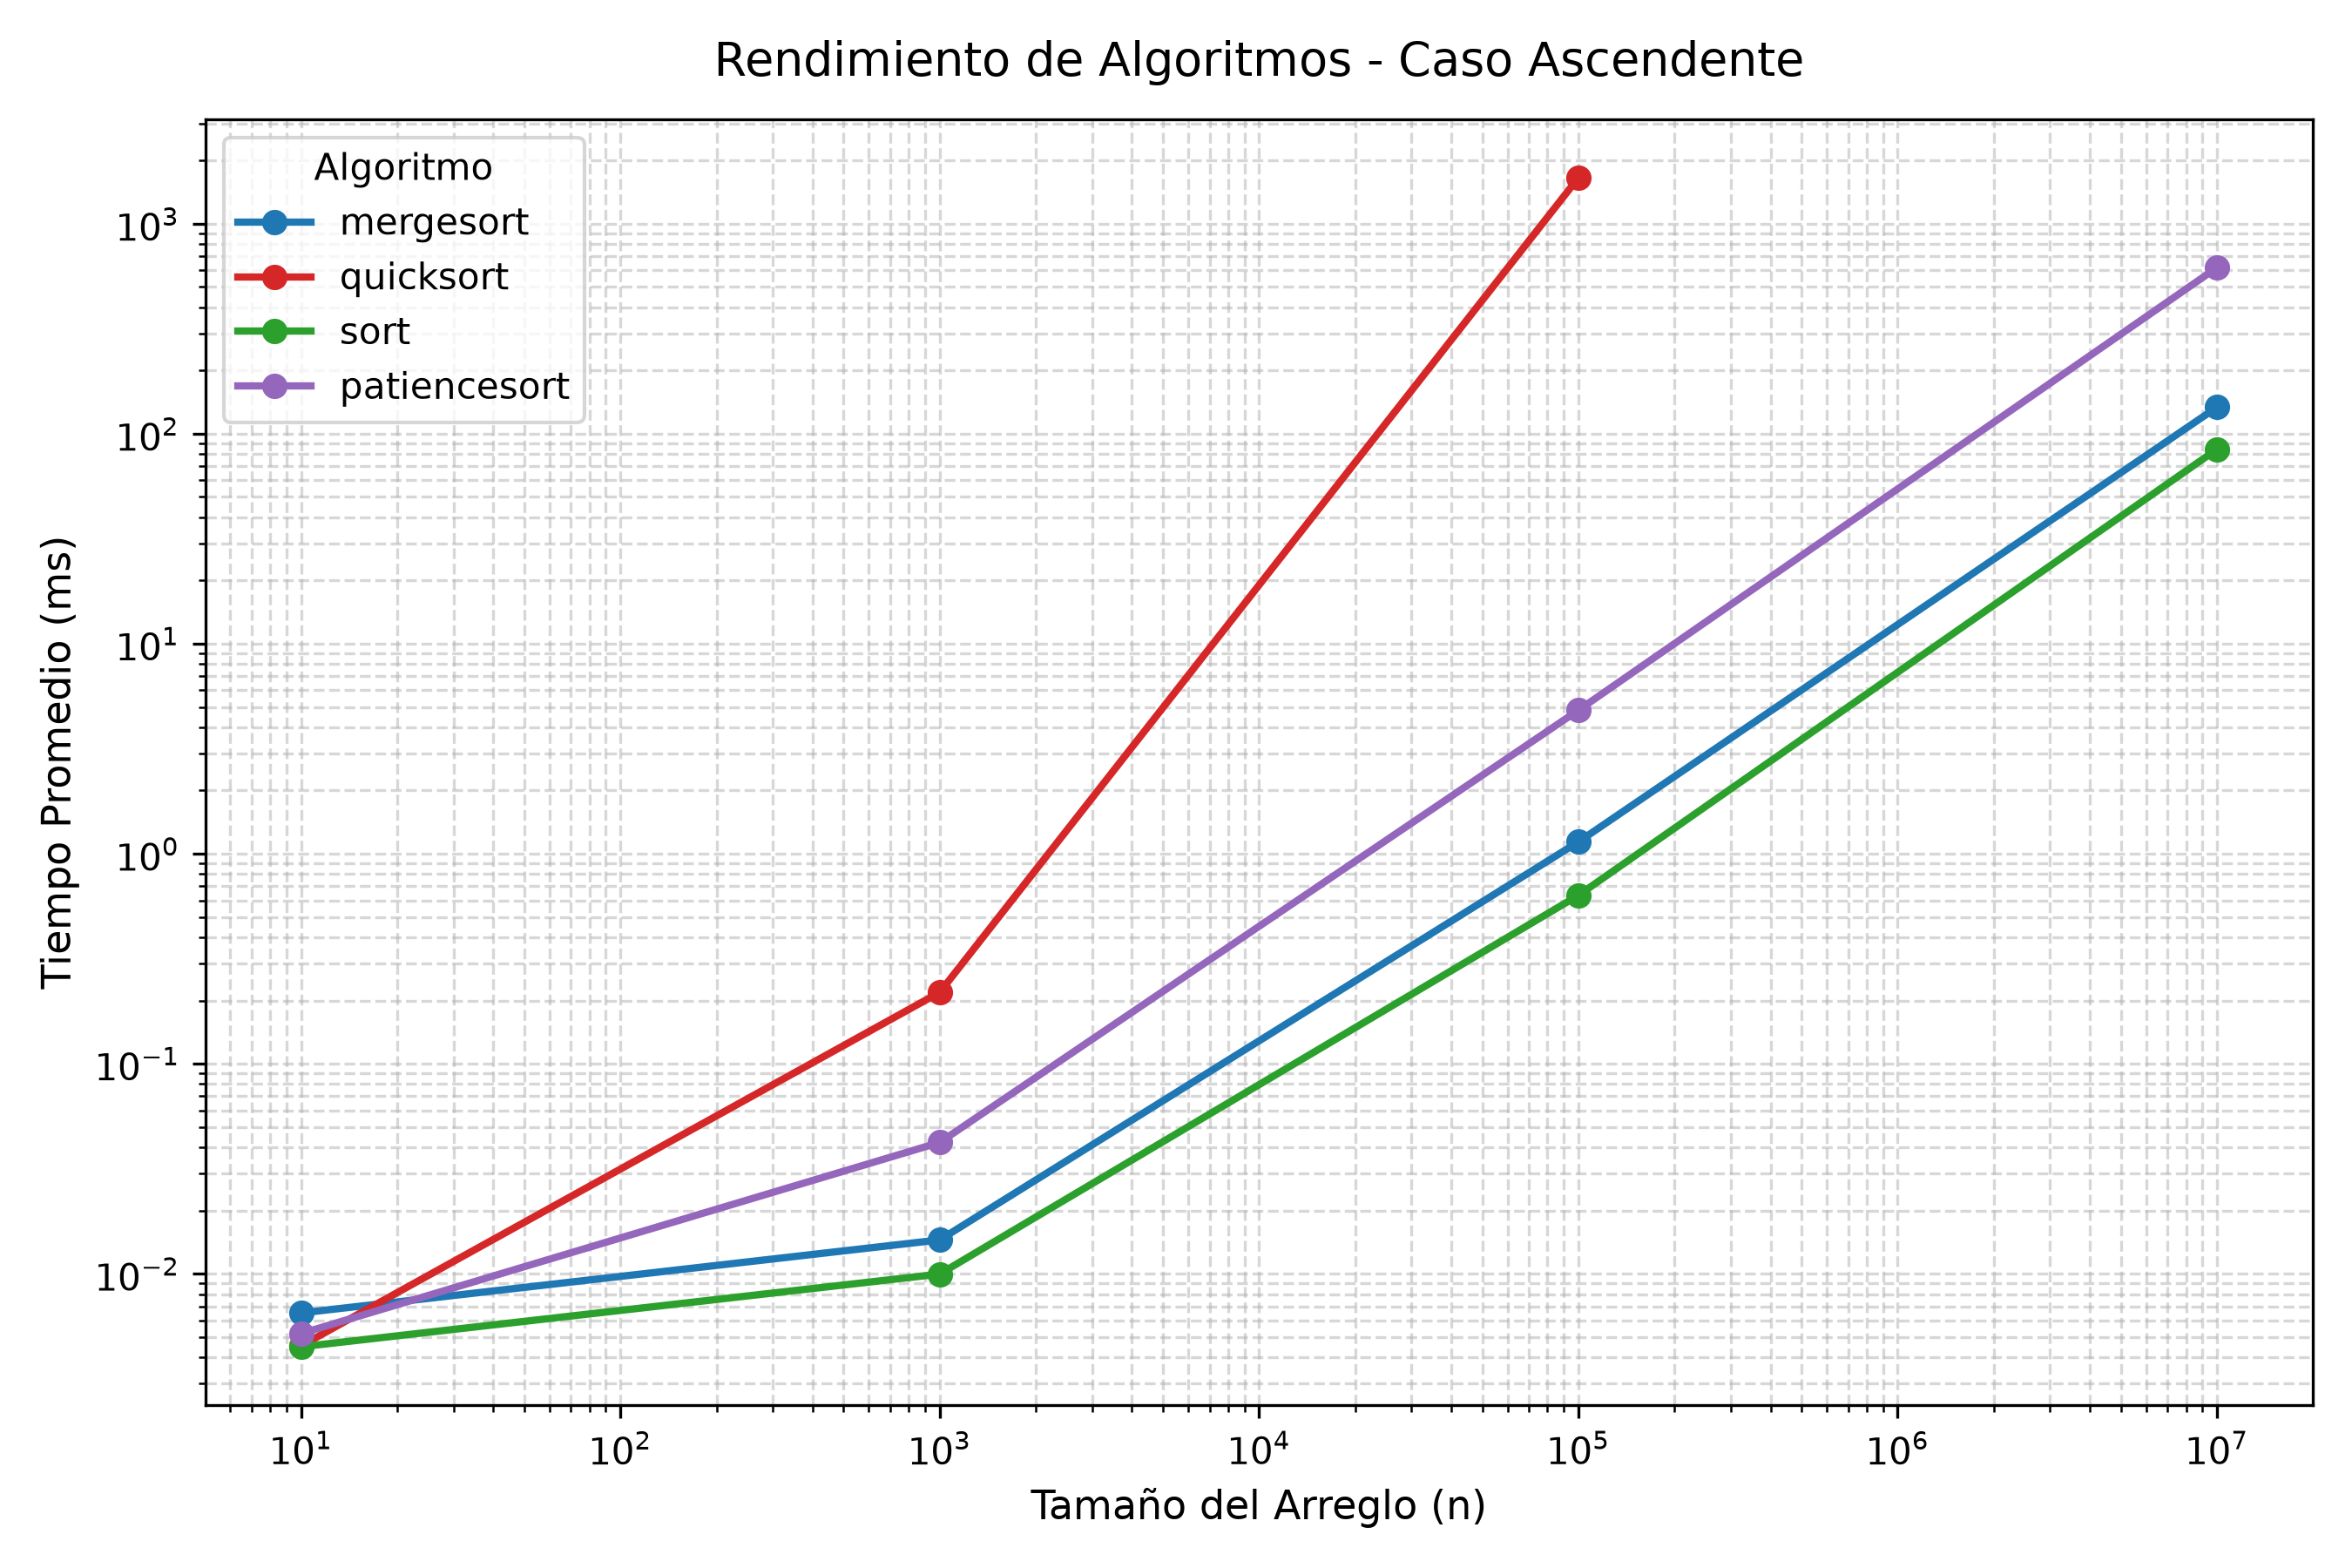
\includegraphics[width=\textwidth]{figures/comparativa_ascendente.png}
        \caption{Ascendente.}
    \end{minipage}\hfill
    \begin{minipage}{0.32\textwidth}
        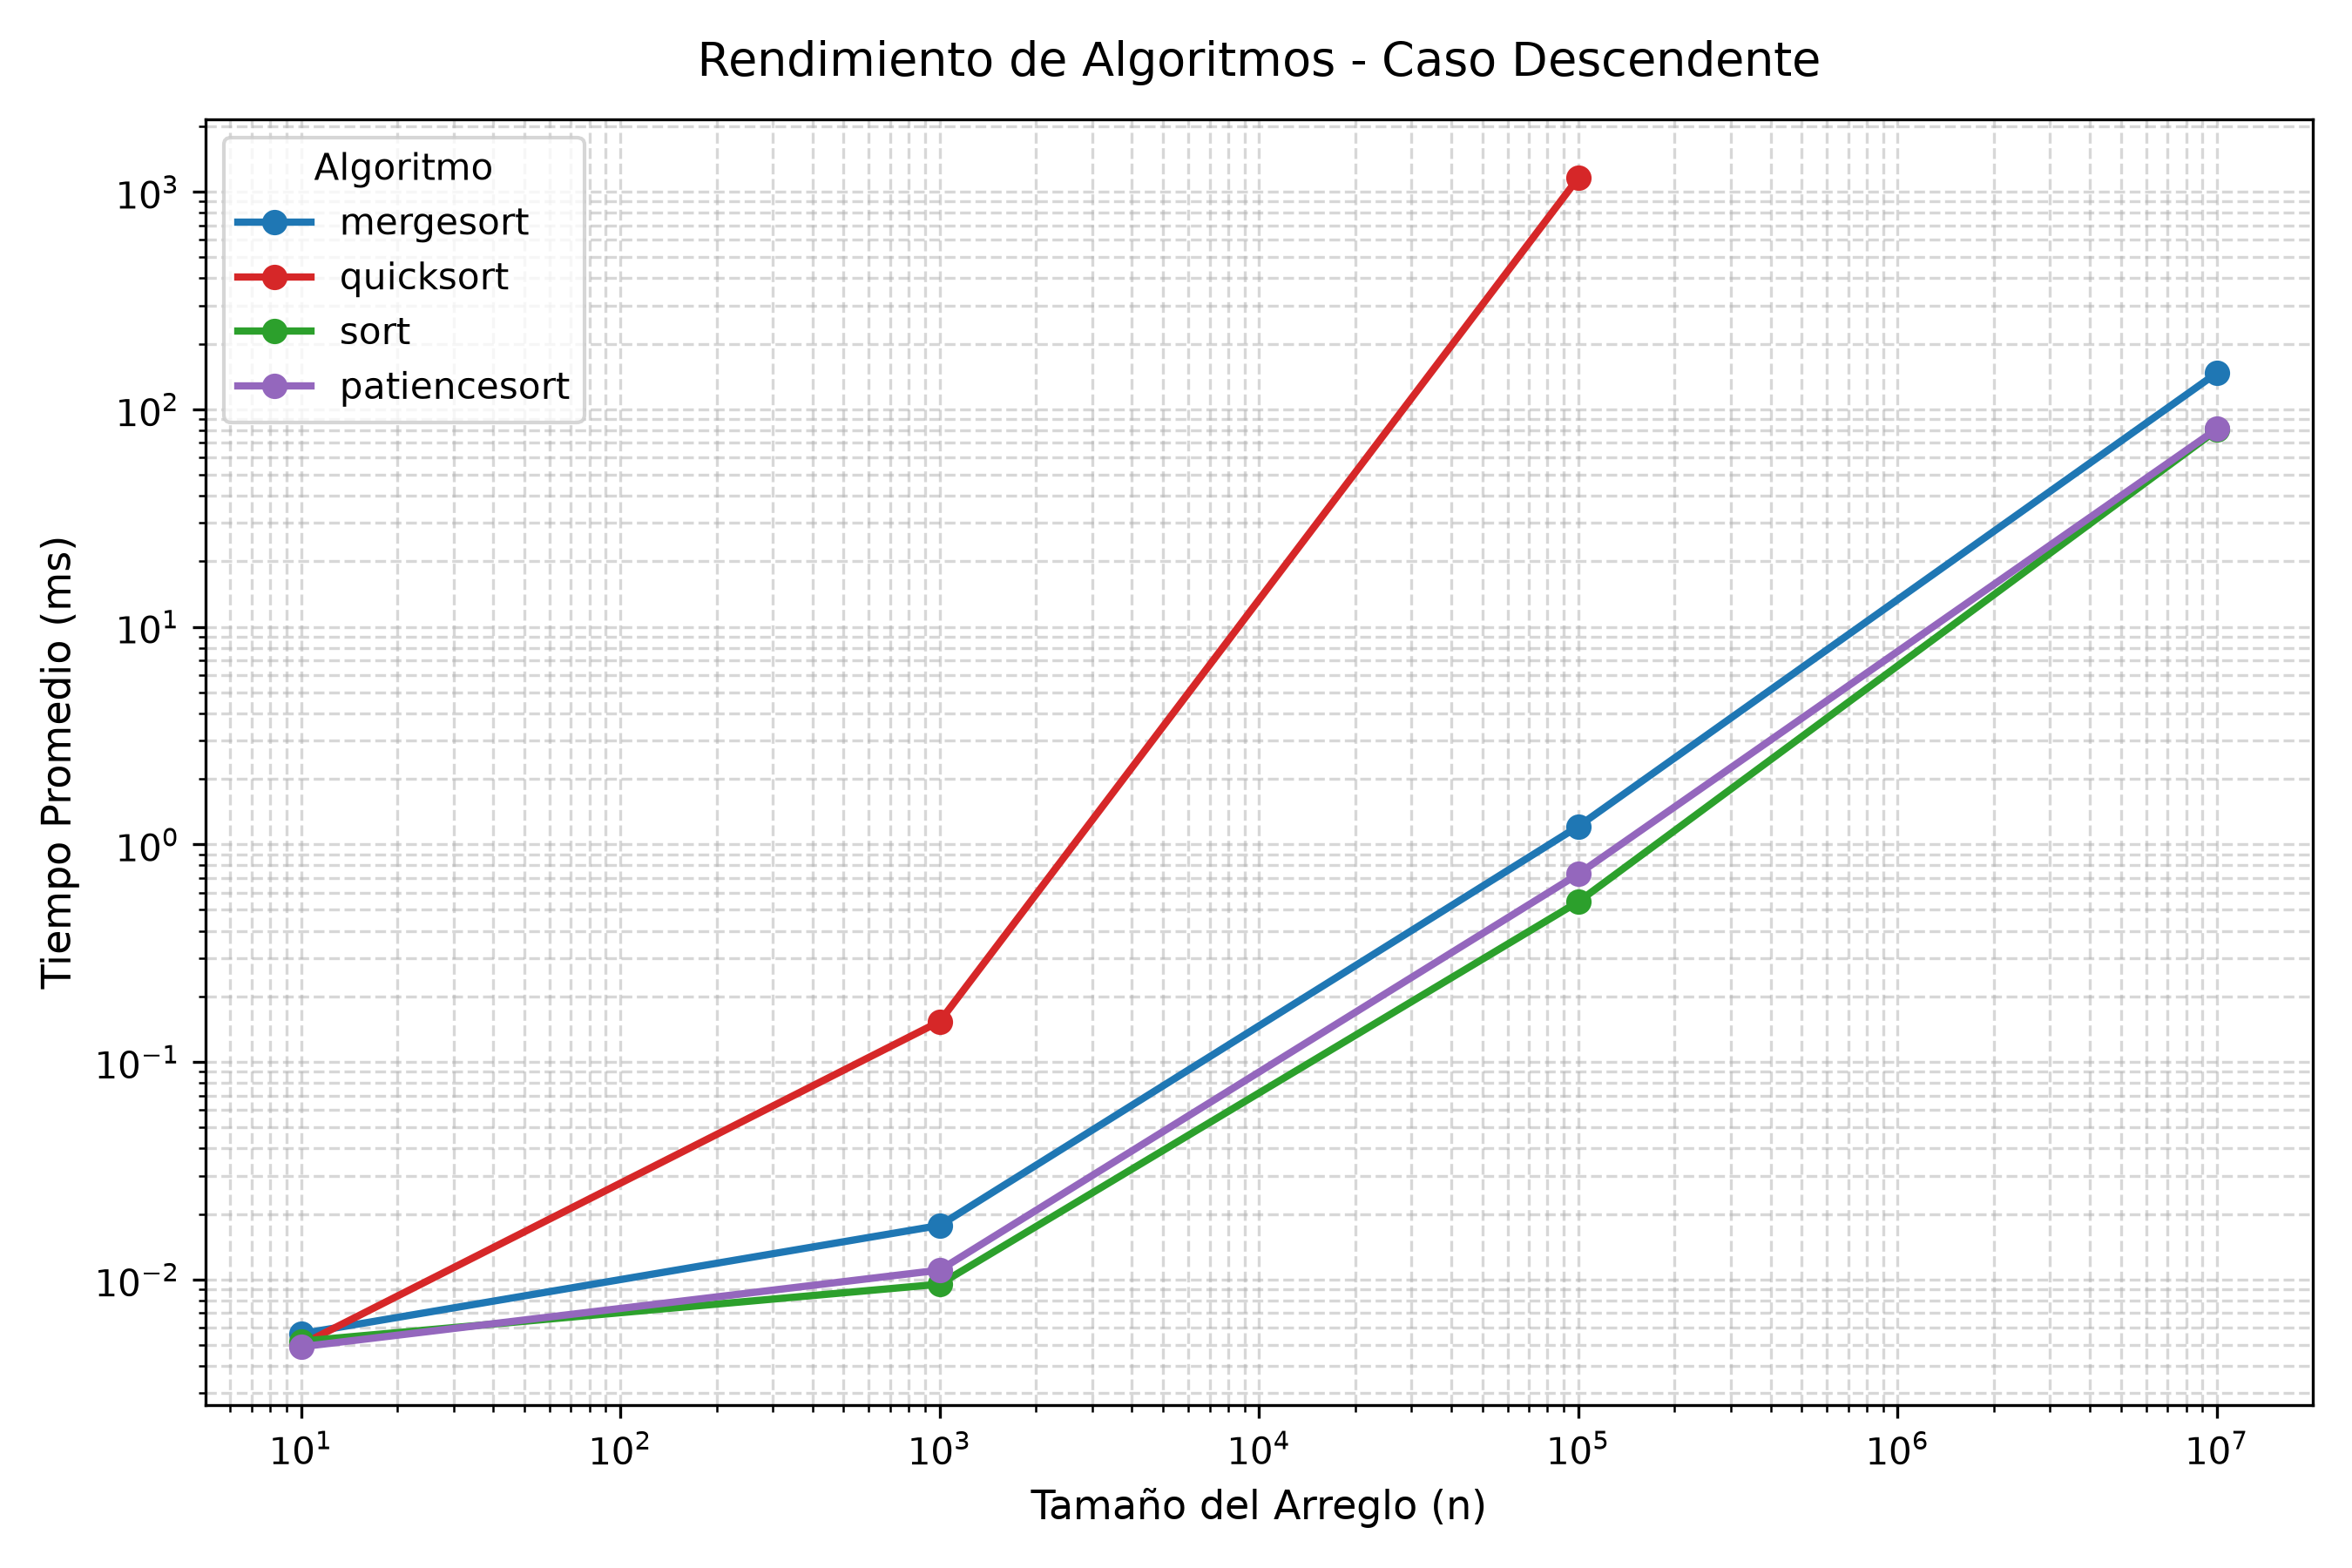
\includegraphics[width=\textwidth]{figures/comparativa_descendente.png}
        \caption{Descendente.}
    \end{minipage}\hfill
    \begin{minipage}{0.32\textwidth}
        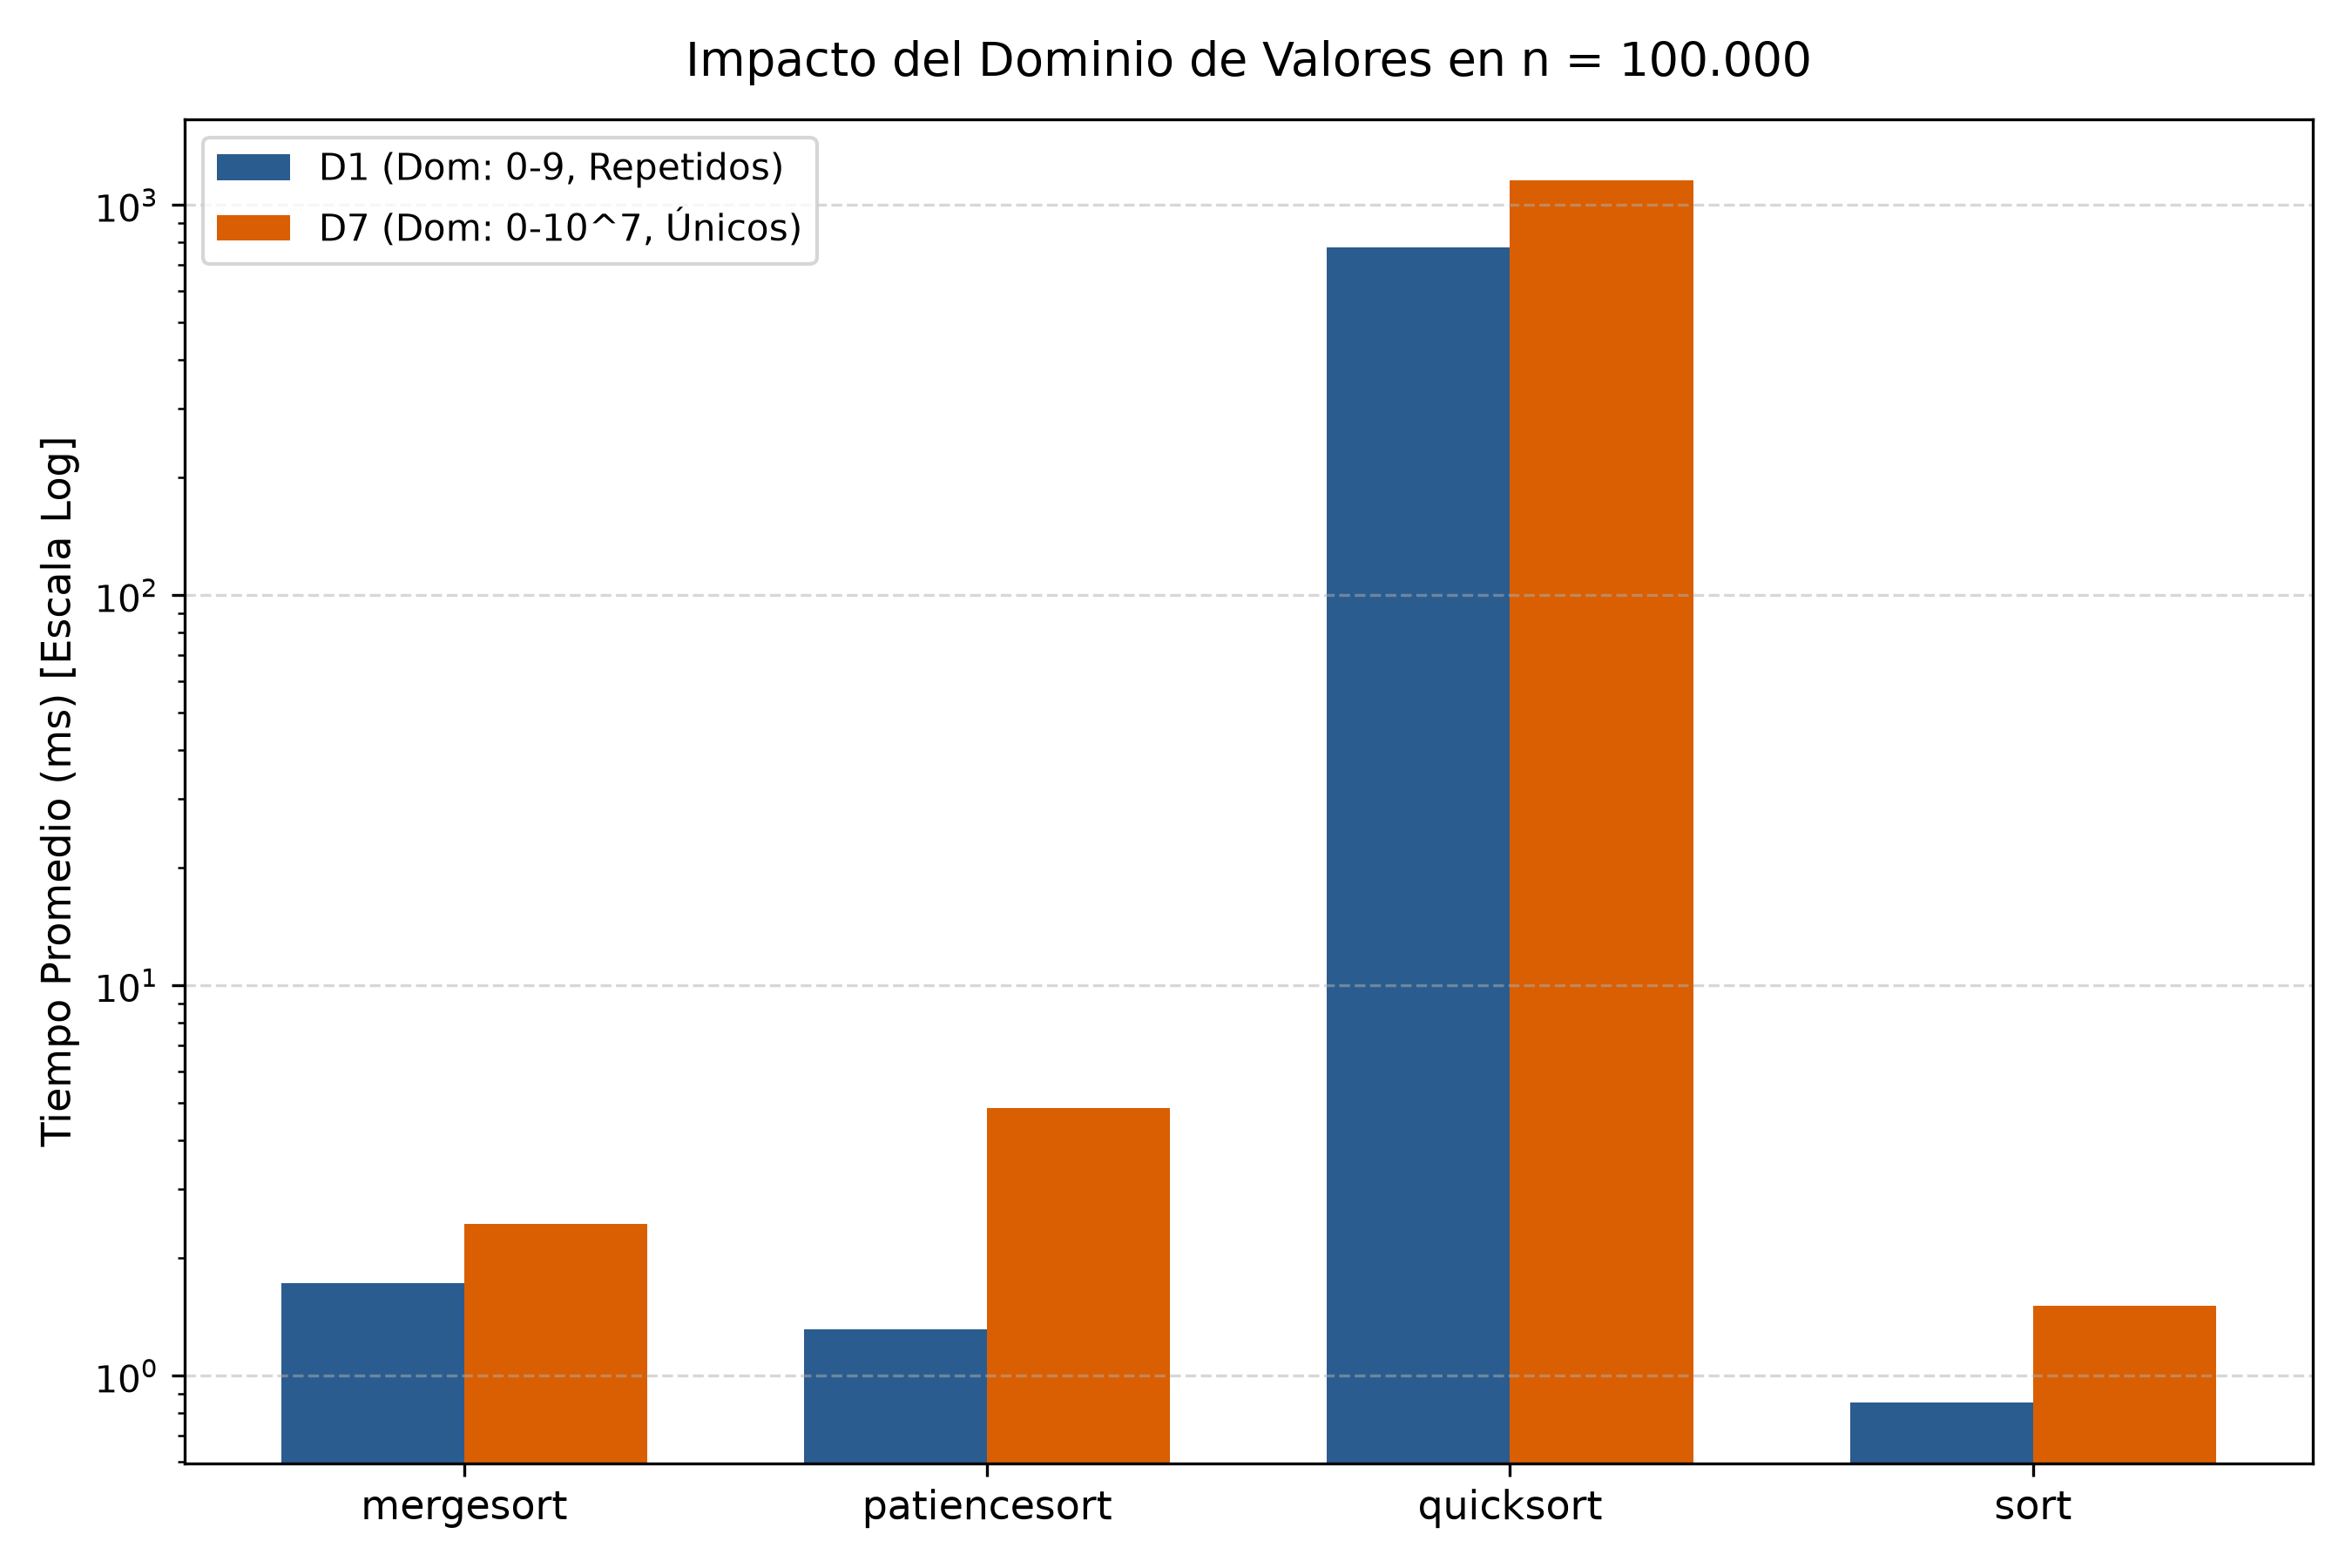
\includegraphics[width=\textwidth]{figures/comparativa_dominios_n100k.png}
        \caption{Dominio ($10^5$).}
    \end{minipage}
\end{figure}

\subsection{Multiplicación de Matrices}

\begin{figure}[H]
    \centering
    \begin{minipage}{0.48\textwidth}
        \centering
        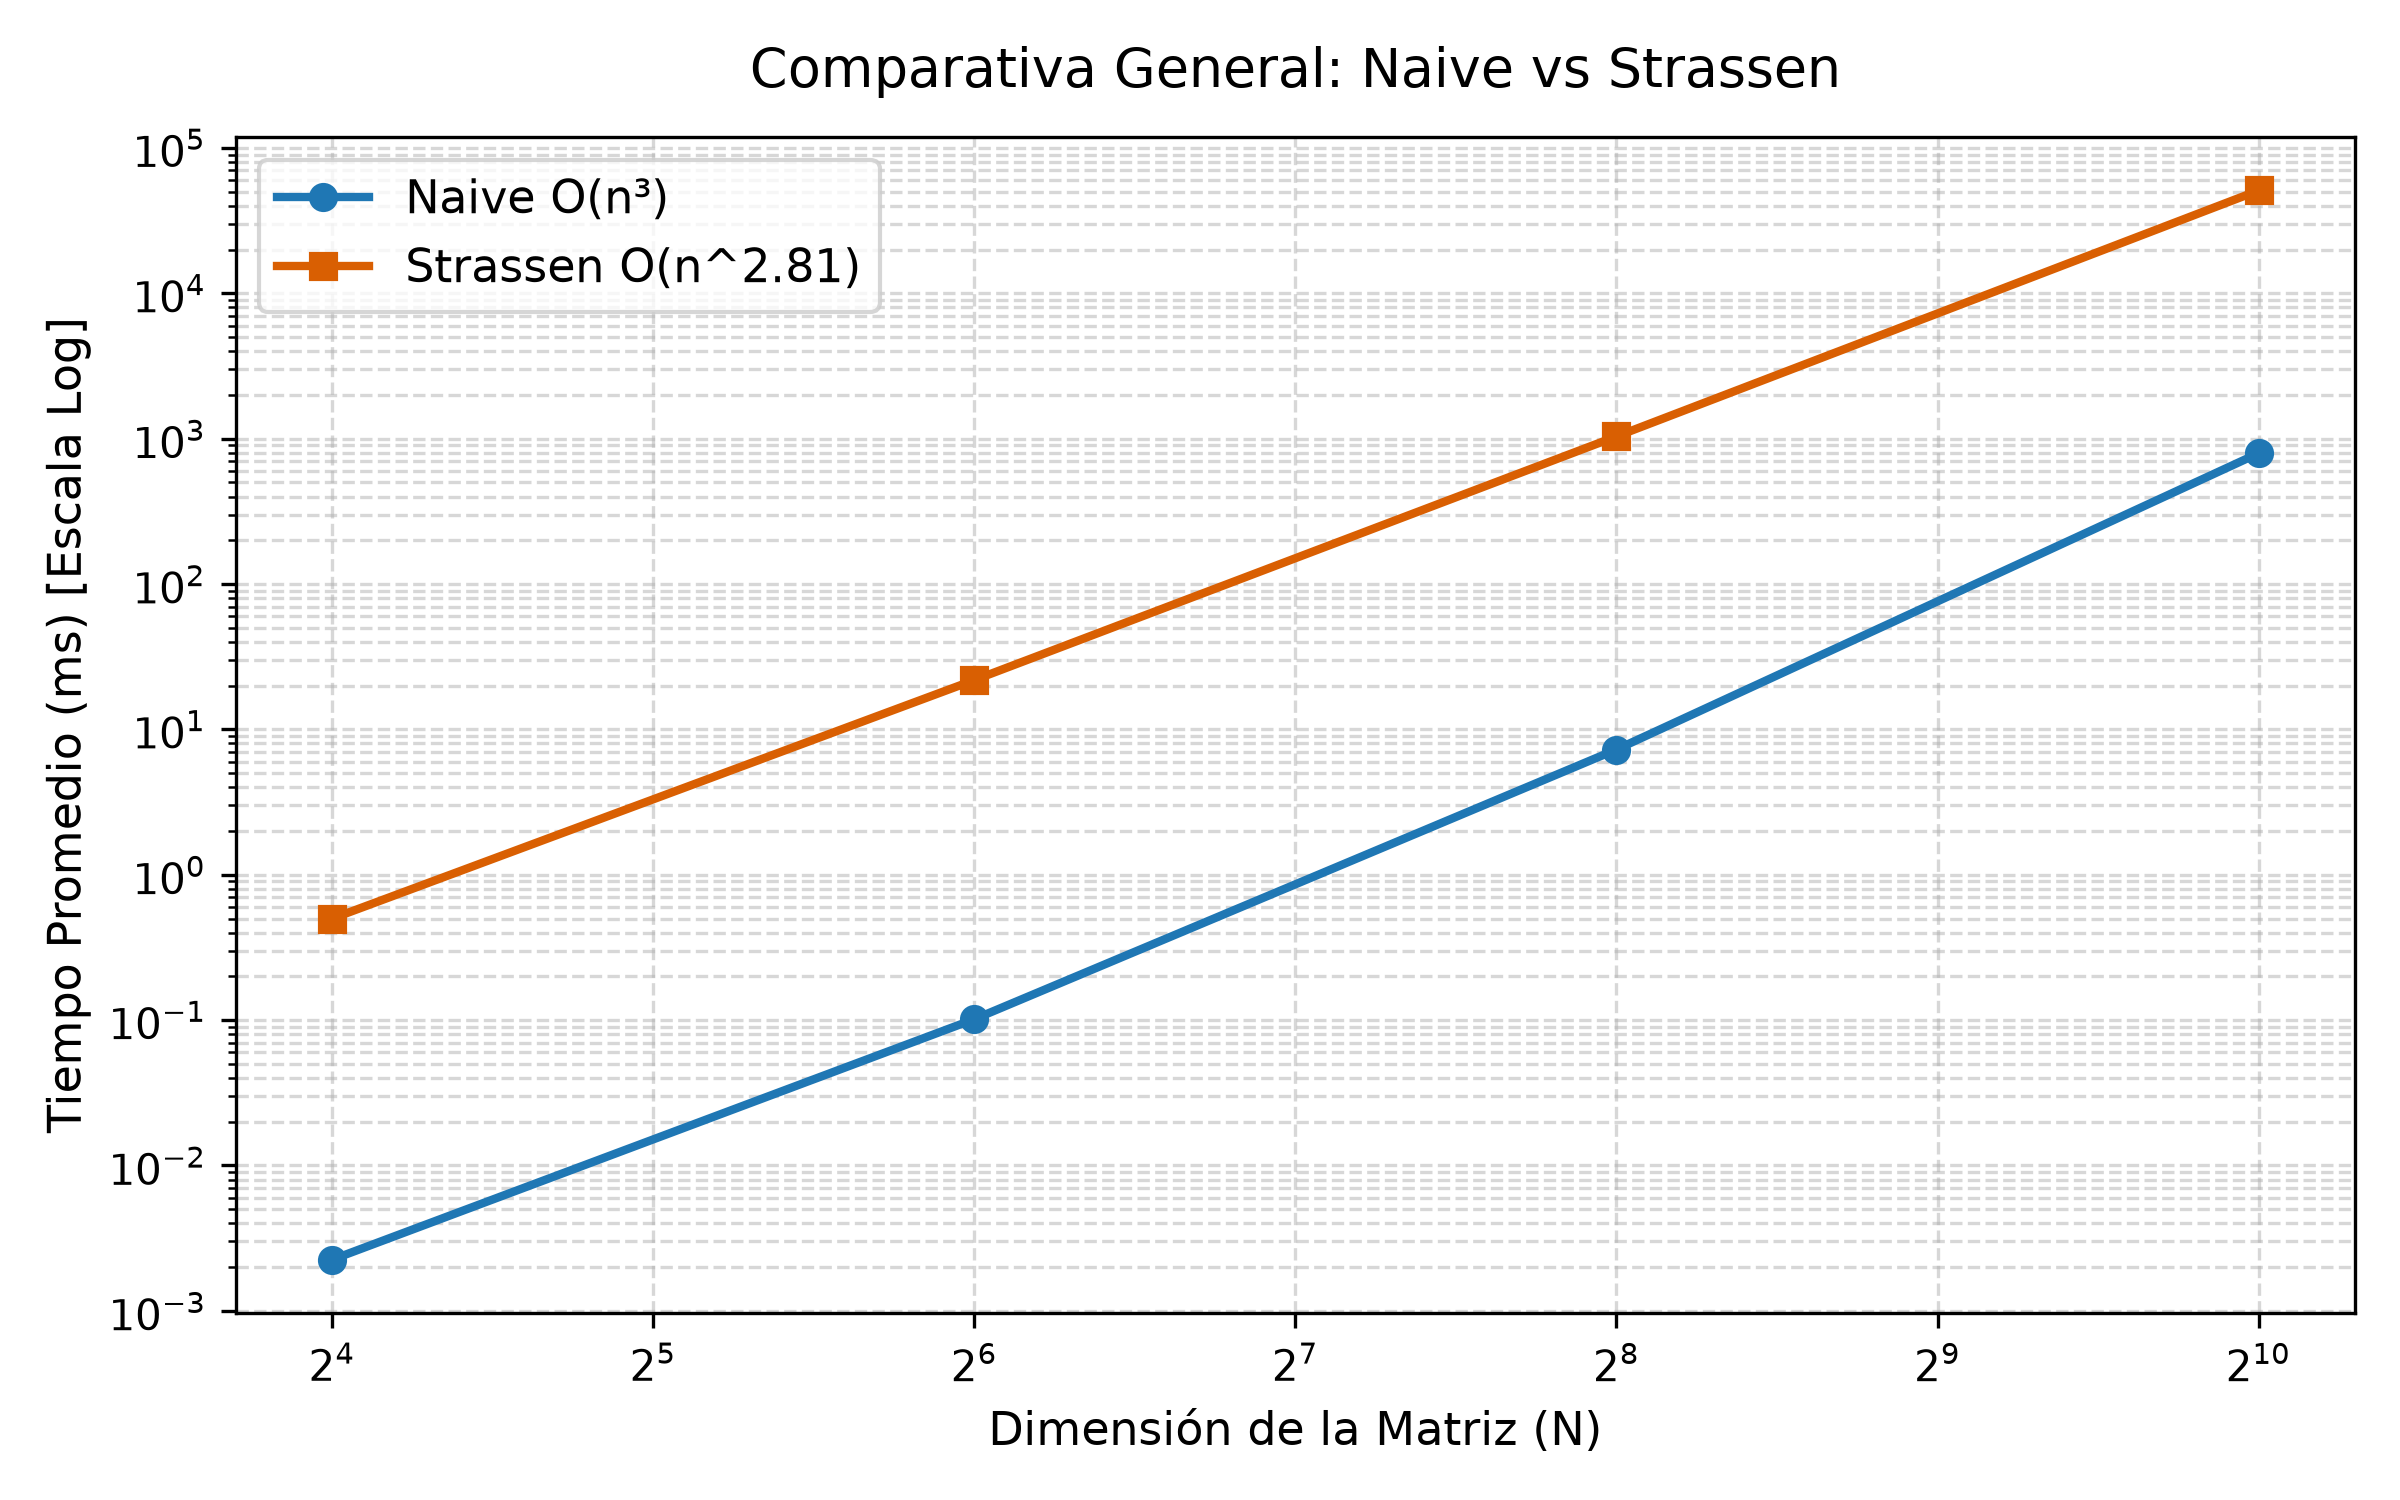
\includegraphics[width=\textwidth]{figures/comparativa_global_matrices.png}
        \caption{Tiempo: Naive vs Strassen.}
        \label{fig:t_matrices}
    \end{minipage}\hfill
    \begin{minipage}{0.48\textwidth}
        \centering
        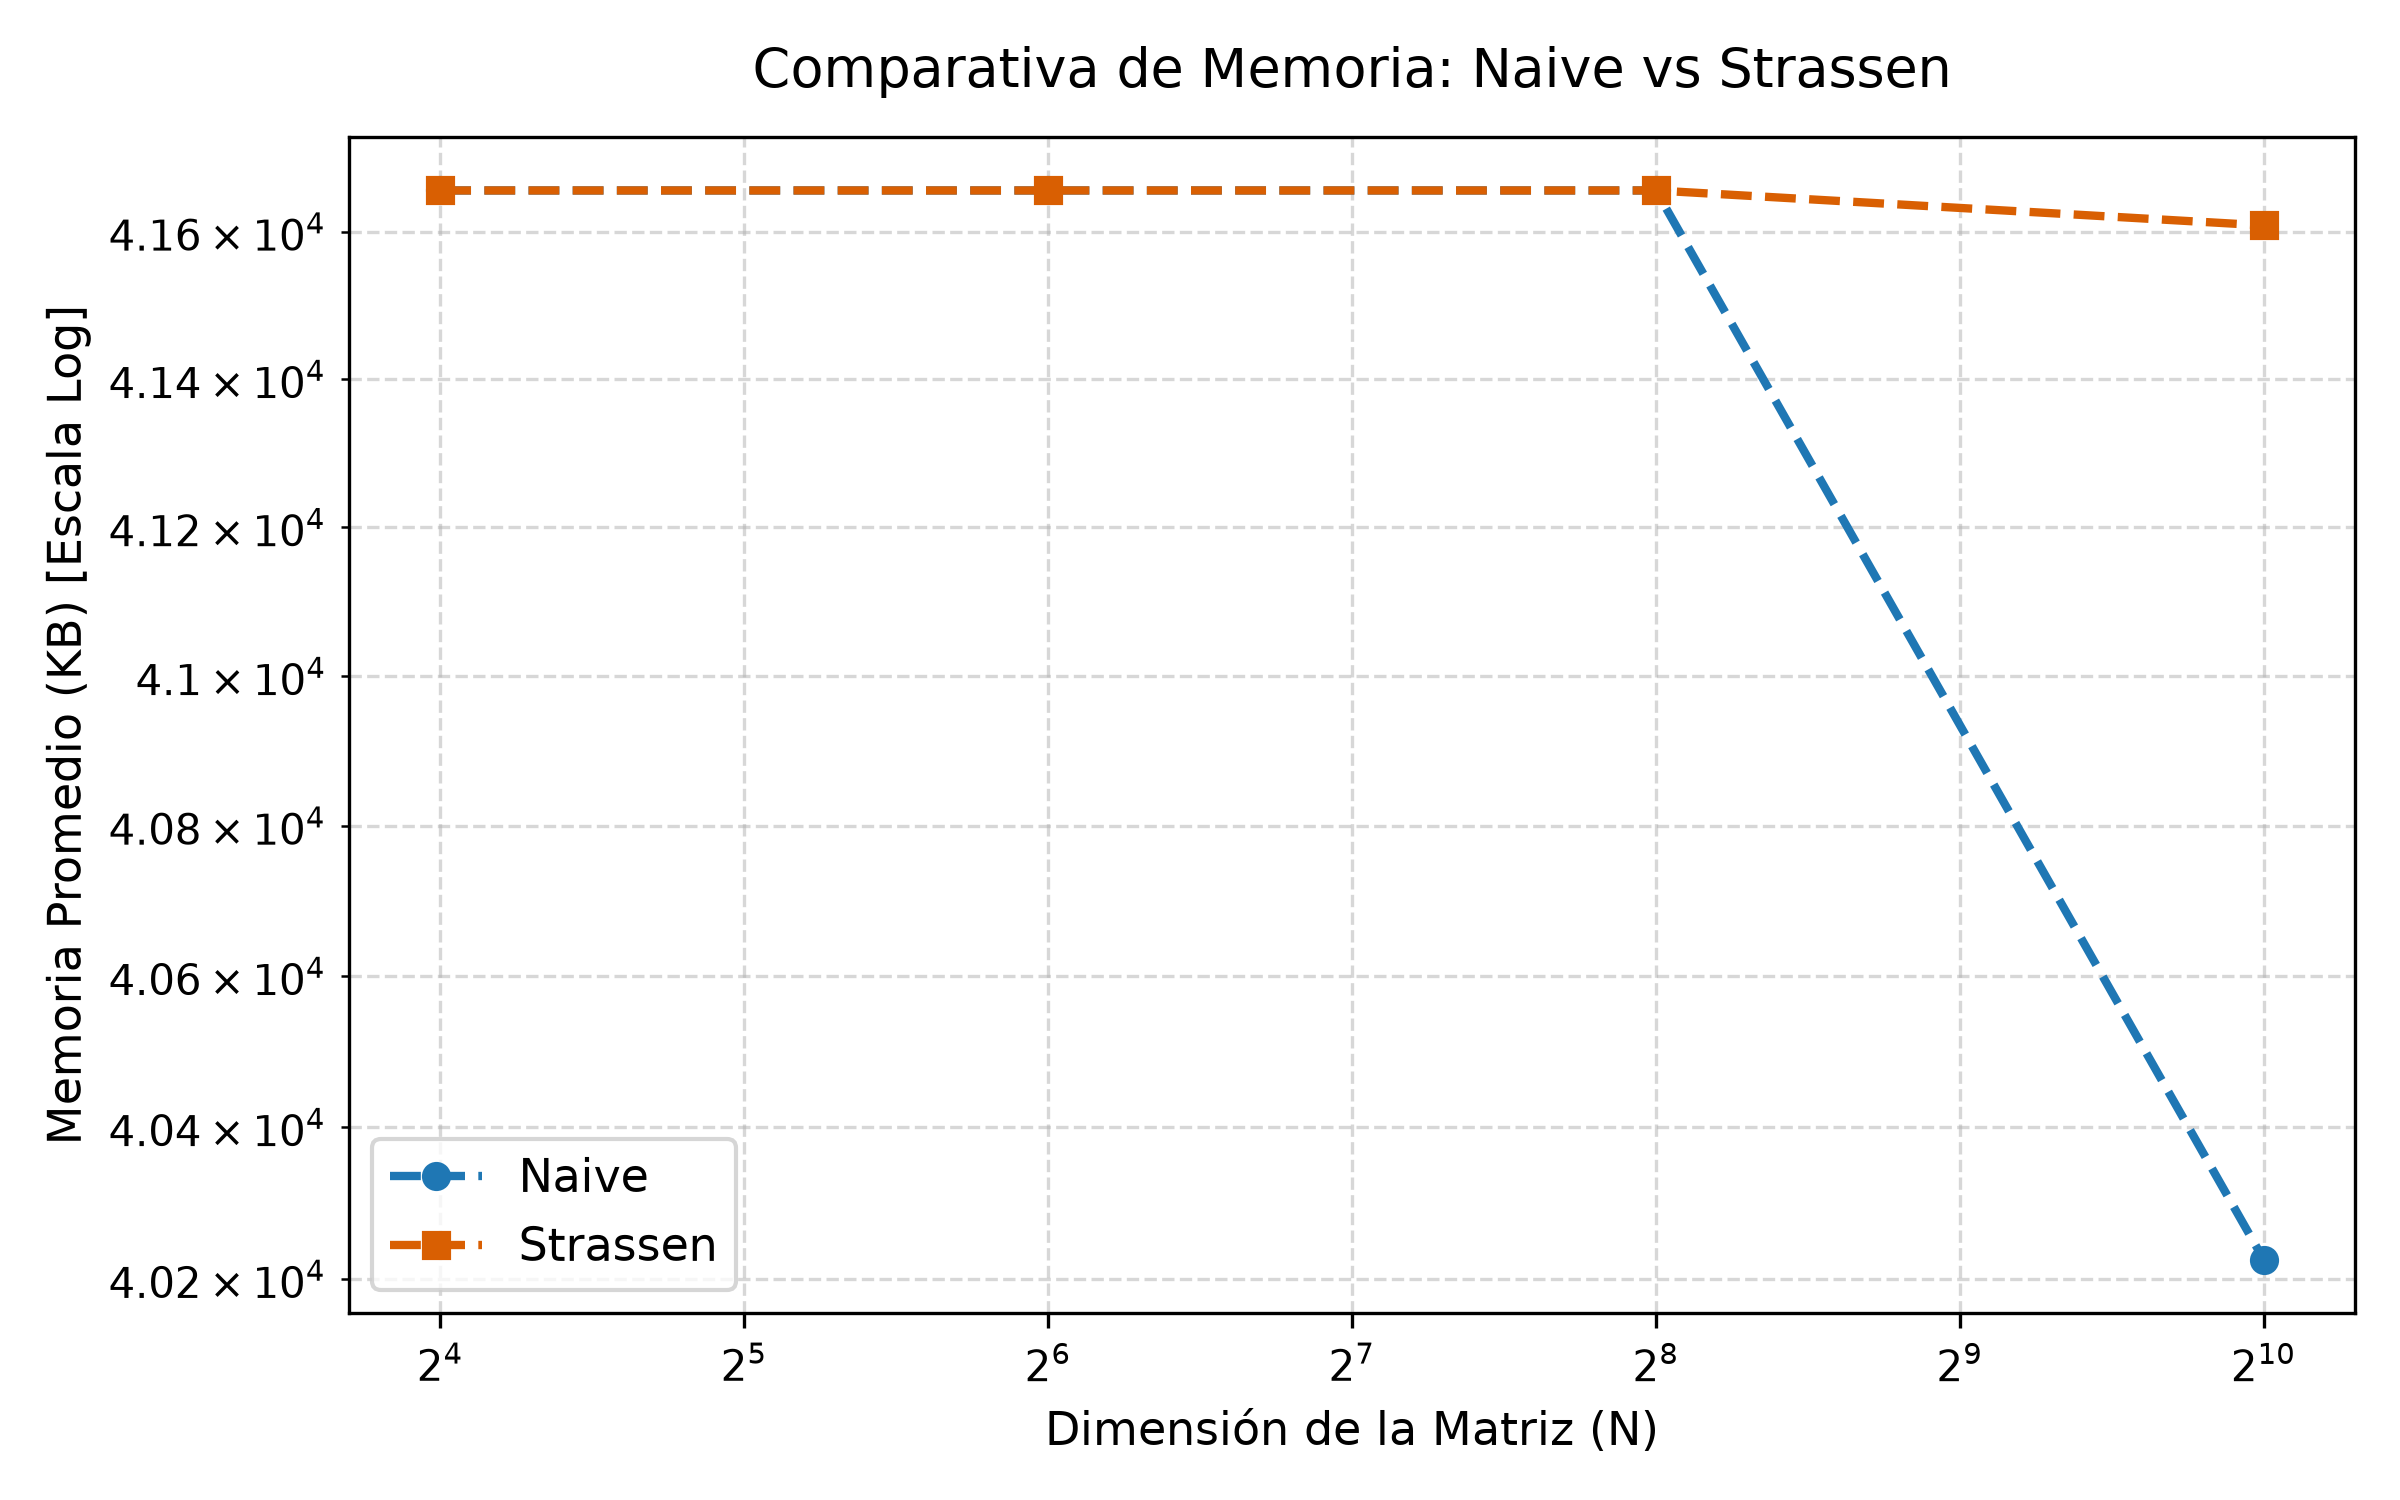
\includegraphics[width=\textwidth]{figures/memoria_global_matrices.png}
        \caption{Memoria: Naive vs Strassen.}
        \label{fig:m_matrices}
    \end{minipage}
\end{figure}

Naive supera por órdenes de magnitud a Strassen (Figura \ref{fig:t_matrices}). La recursividad profunda en $N=1024$ genera $\approx 3.29 \times 10^8$ llamadas, asfixiando la ganancia asintótica por el inmenso \textit{overhead}. Esto se refleja en la Figura \ref{fig:m_matrices}: Strassen exige una asignación masiva en el \textit{heap}, mientras Naive mantiene una huella estable $\mathcal{O}(N^2)$. El tiempo demostró ser agnóstico a la estructura y dominio de las matrices, ya que ninguna implementación omite cálculos sobre ceros.

\begin{figure}[H]
    \centering
    \begin{minipage}{0.48\textwidth}
        \centering
        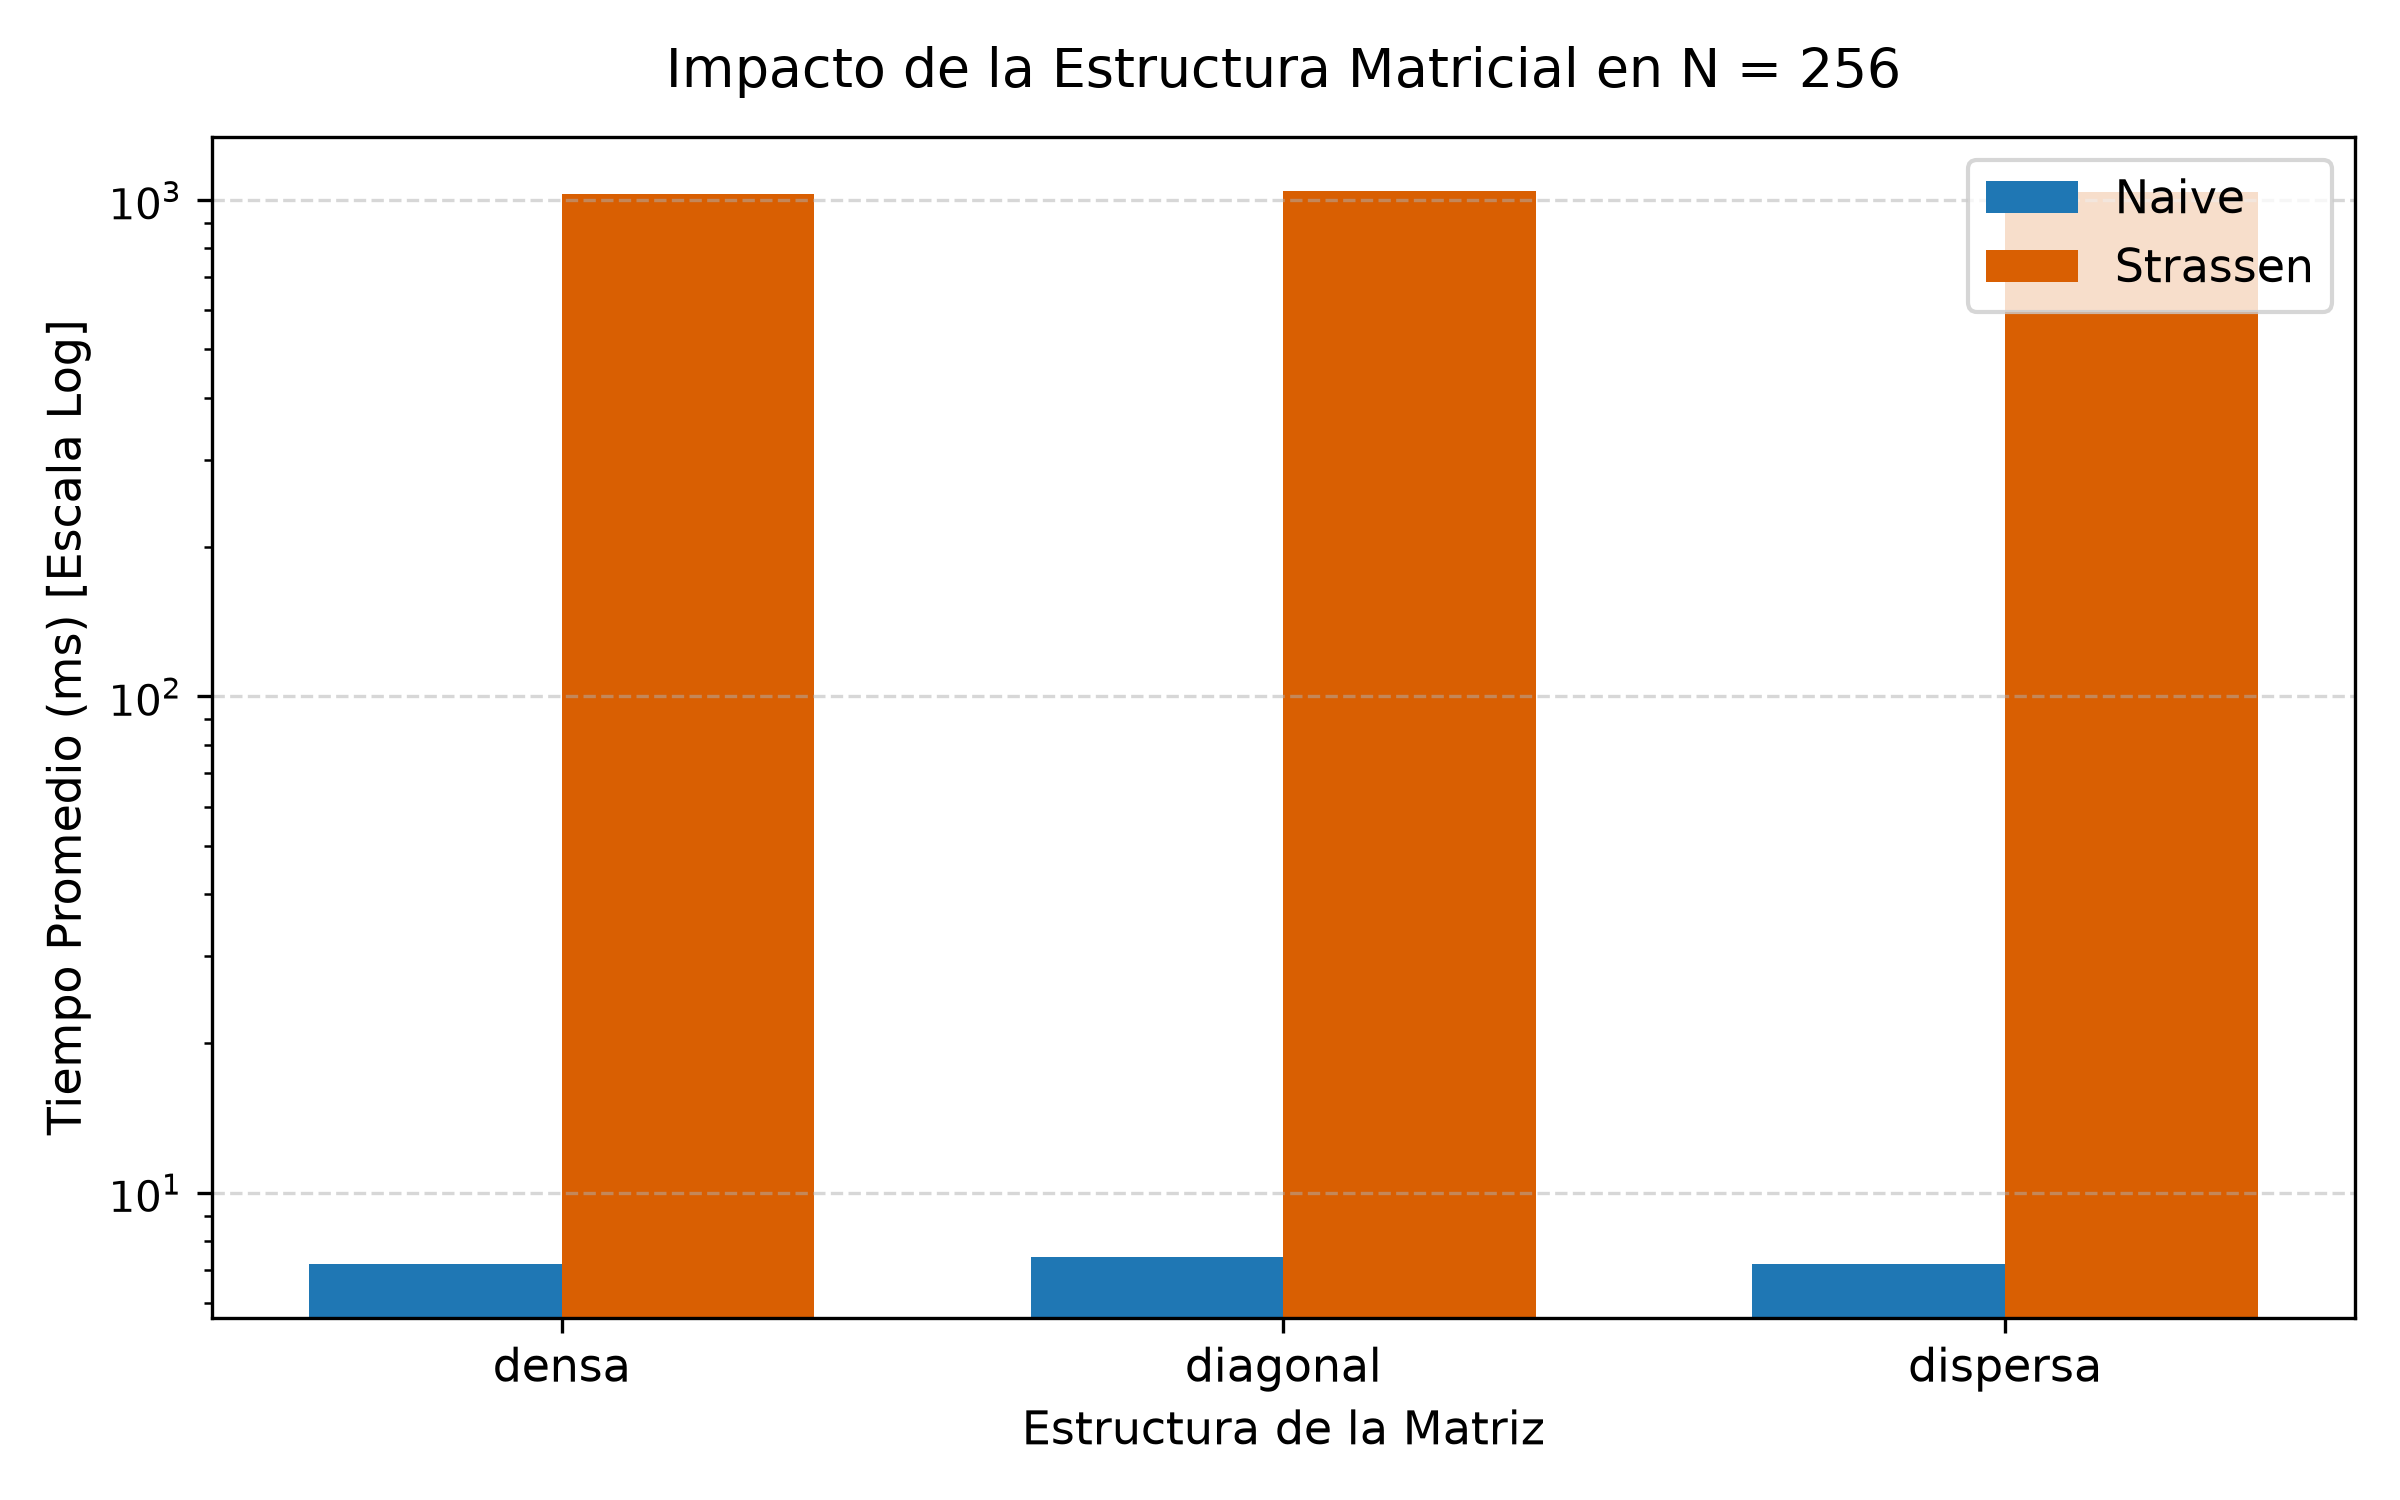
\includegraphics[width=\textwidth]{figures/impacto_tipo_matrices.png}
        \caption{Estructura interna.}
    \end{minipage}\hfill
    \begin{minipage}{0.48\textwidth}
        \centering
        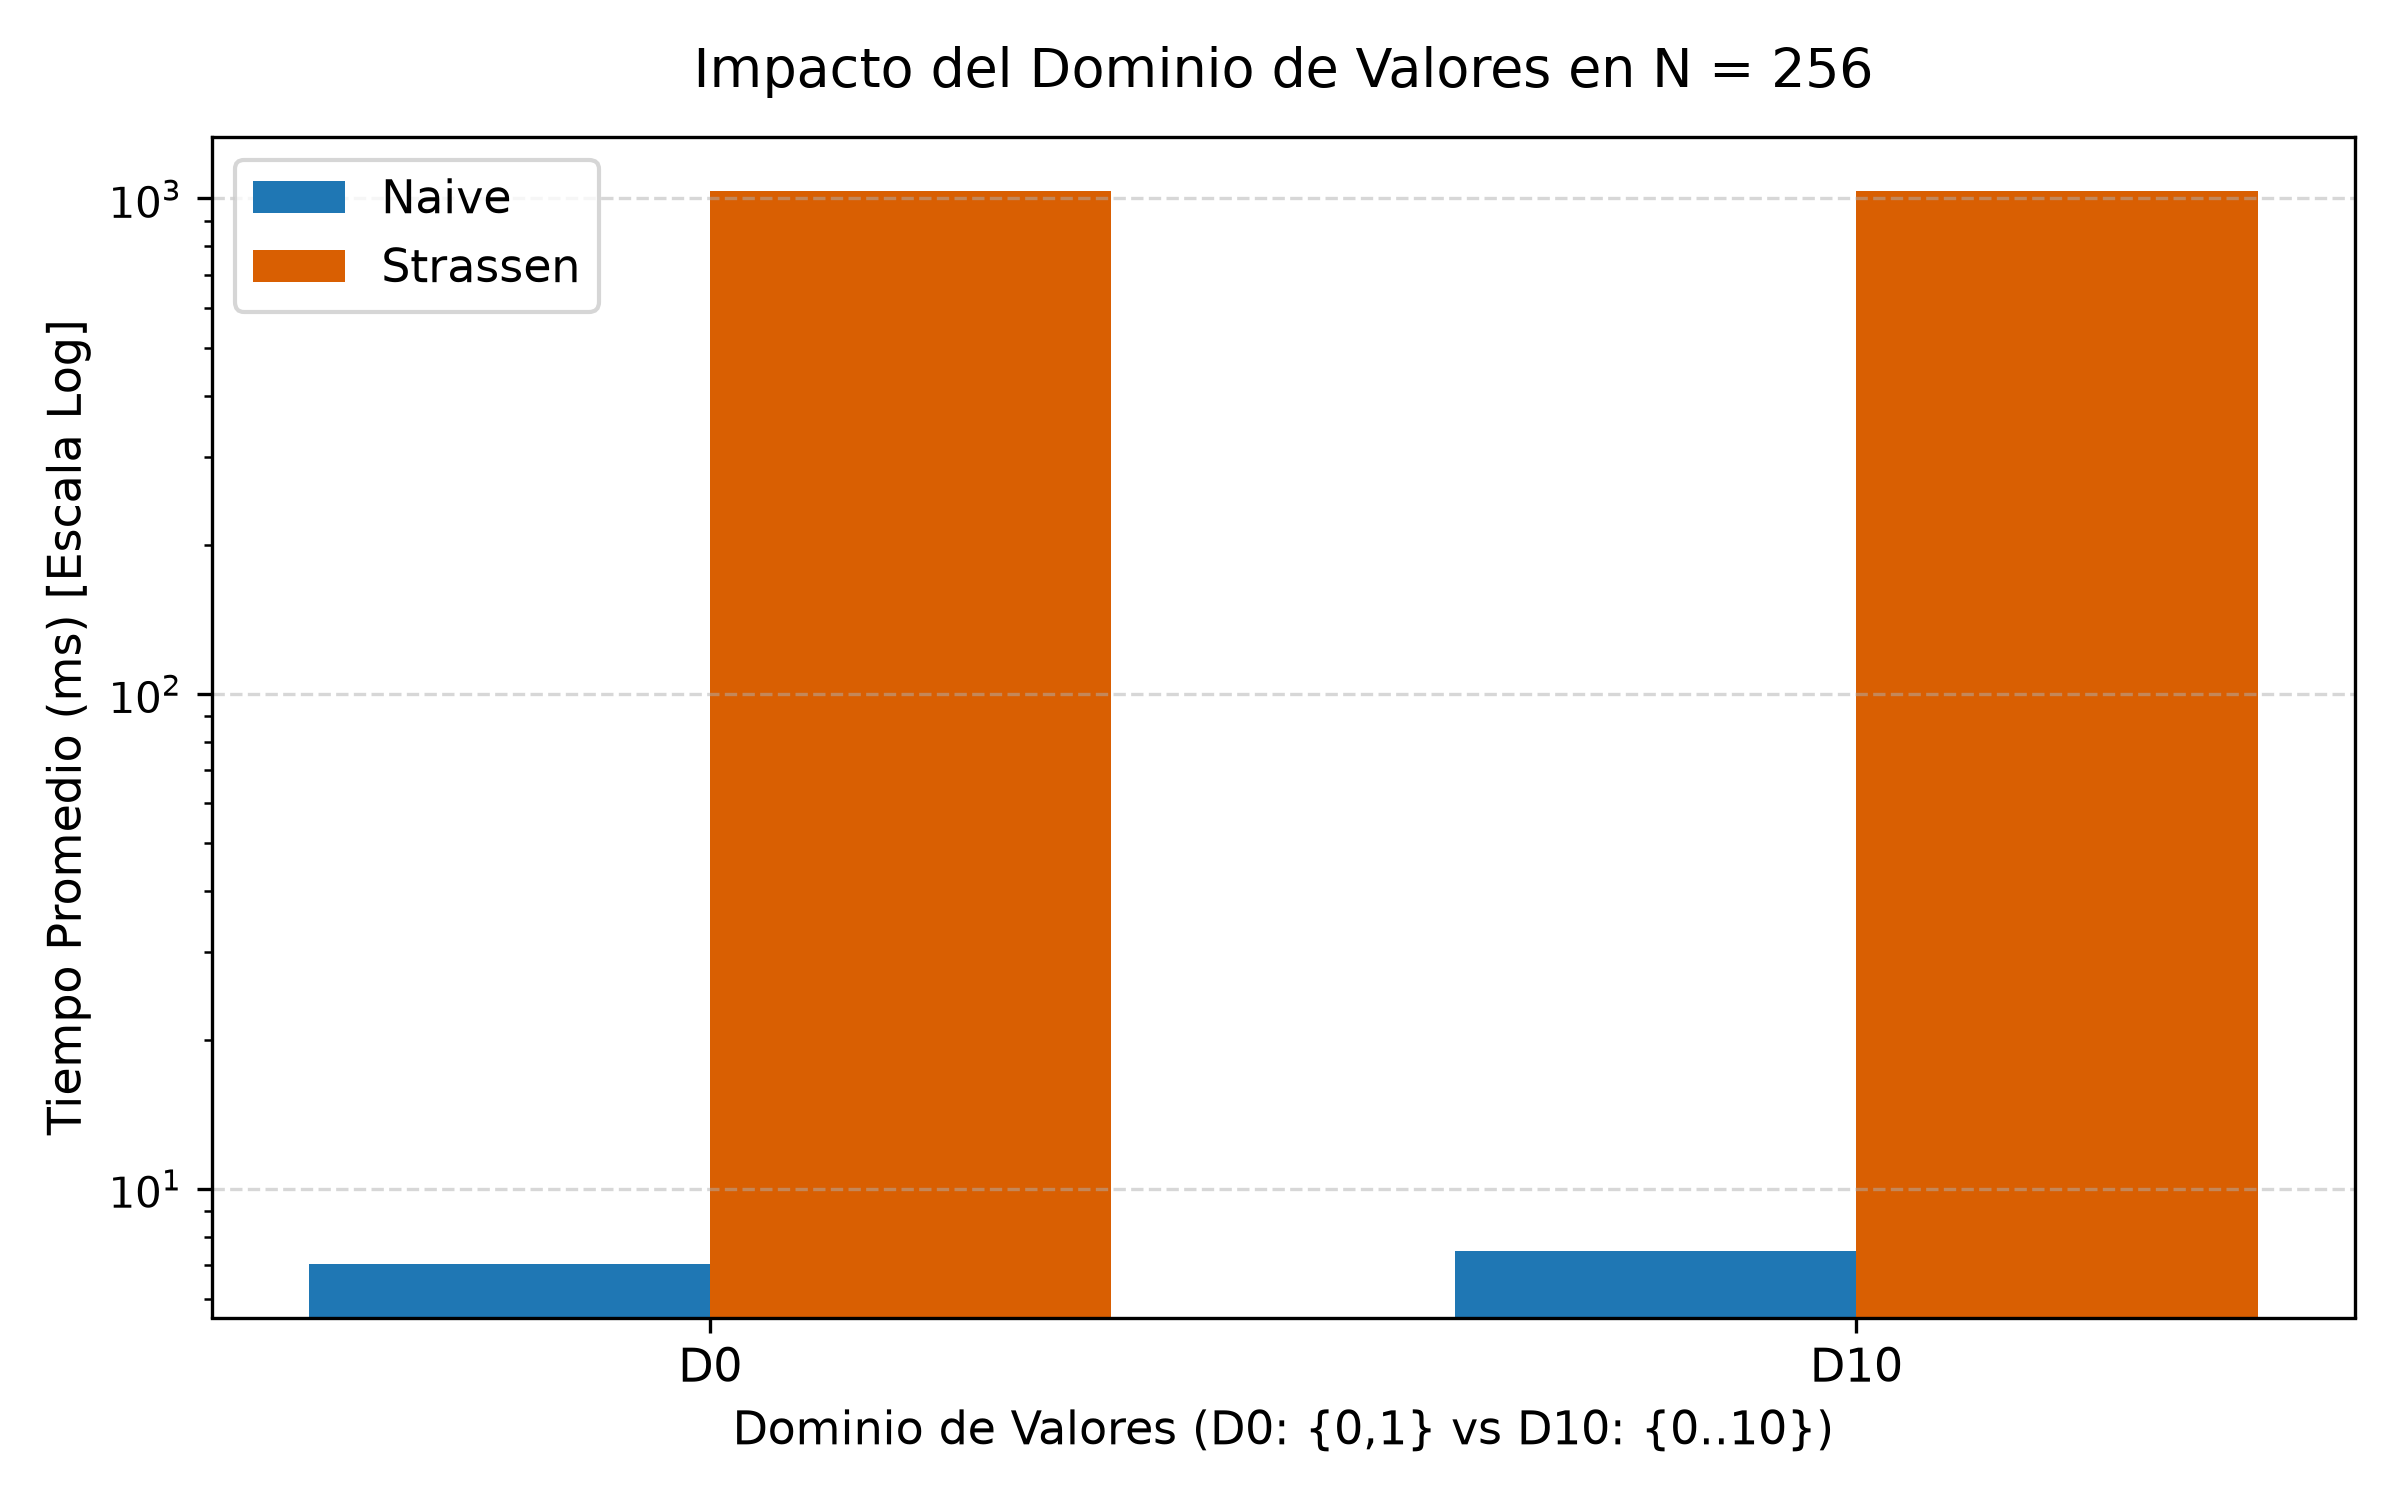
\includegraphics[width=\textwidth]{figures/impacto_dominio_matrices.png}
        \caption{Dominio numérico.}
    \end{minipage}
\end{figure}

\section{Conclusiones}
Los resultados demuestran que la notación asintótica teórica es insuficiente para dictaminar el desempeño en plataformas de cómputo reales. En ordenamiento, la topología inicial del arreglo condiciona la simetría de partición en \texttt{QuickSort} y el número de pilas en \texttt{PatienceSort}, demostrando la robustez de algoritmos con cotas asintóticas garantizadas como \texttt{MergeSort} e híbridos introspectivos como \texttt{std::sort}. En multiplicación matricial, la ventaja teórica de Strassen ($\mathcal{O}(N^{2.81})$) es neutralizada para dimensiones prácticas ($N \le 1024$) debido al costo de gestión de memoria dinámica en el \textit{heap} y la degradación de la localidad de caché frente a un triple bucle iterativo contiguo vectorizado por el compiladorhola.

\end{document}